% !TEX root = ../STP_Journal.tex
\subsubsection{Robust Trajectory Tracking}
In the planning phase, we reduced the maximum turn rate of the vehicles from $1$ to $0.6$, and the speed range from $[0.5, 1]$ to exactly $0.75$ (constant speed). With these reduced control authorities, we determined from the disturbance rejection phase that a nominal trajectory from the planning phase can be robustly tracked within a distance of $R_{\text{EB}} = 0.075$.

Fig. \ref{fig:rtt_traj} shows vehicle trajectories in the situation where each vehicle robustly tracks a pre-specified trajectory and is guaranteed to stay inside a ``bubble" around the trajectory. Fig. \ref{fig:rtt_rs3} shows the evolution of BRS and induced obstacles for vehicle $\veh_3$. The obstacles induced by other vehicles inhibit the evolution of the BRS, carving out thin ``channels'', which can be seen at $t = -2.59$.%, that separate the BRS into different “islands”. %One can see how these channels and islands form by examining the time evolution of the BRS set.

\begin{figure}
  \centering
  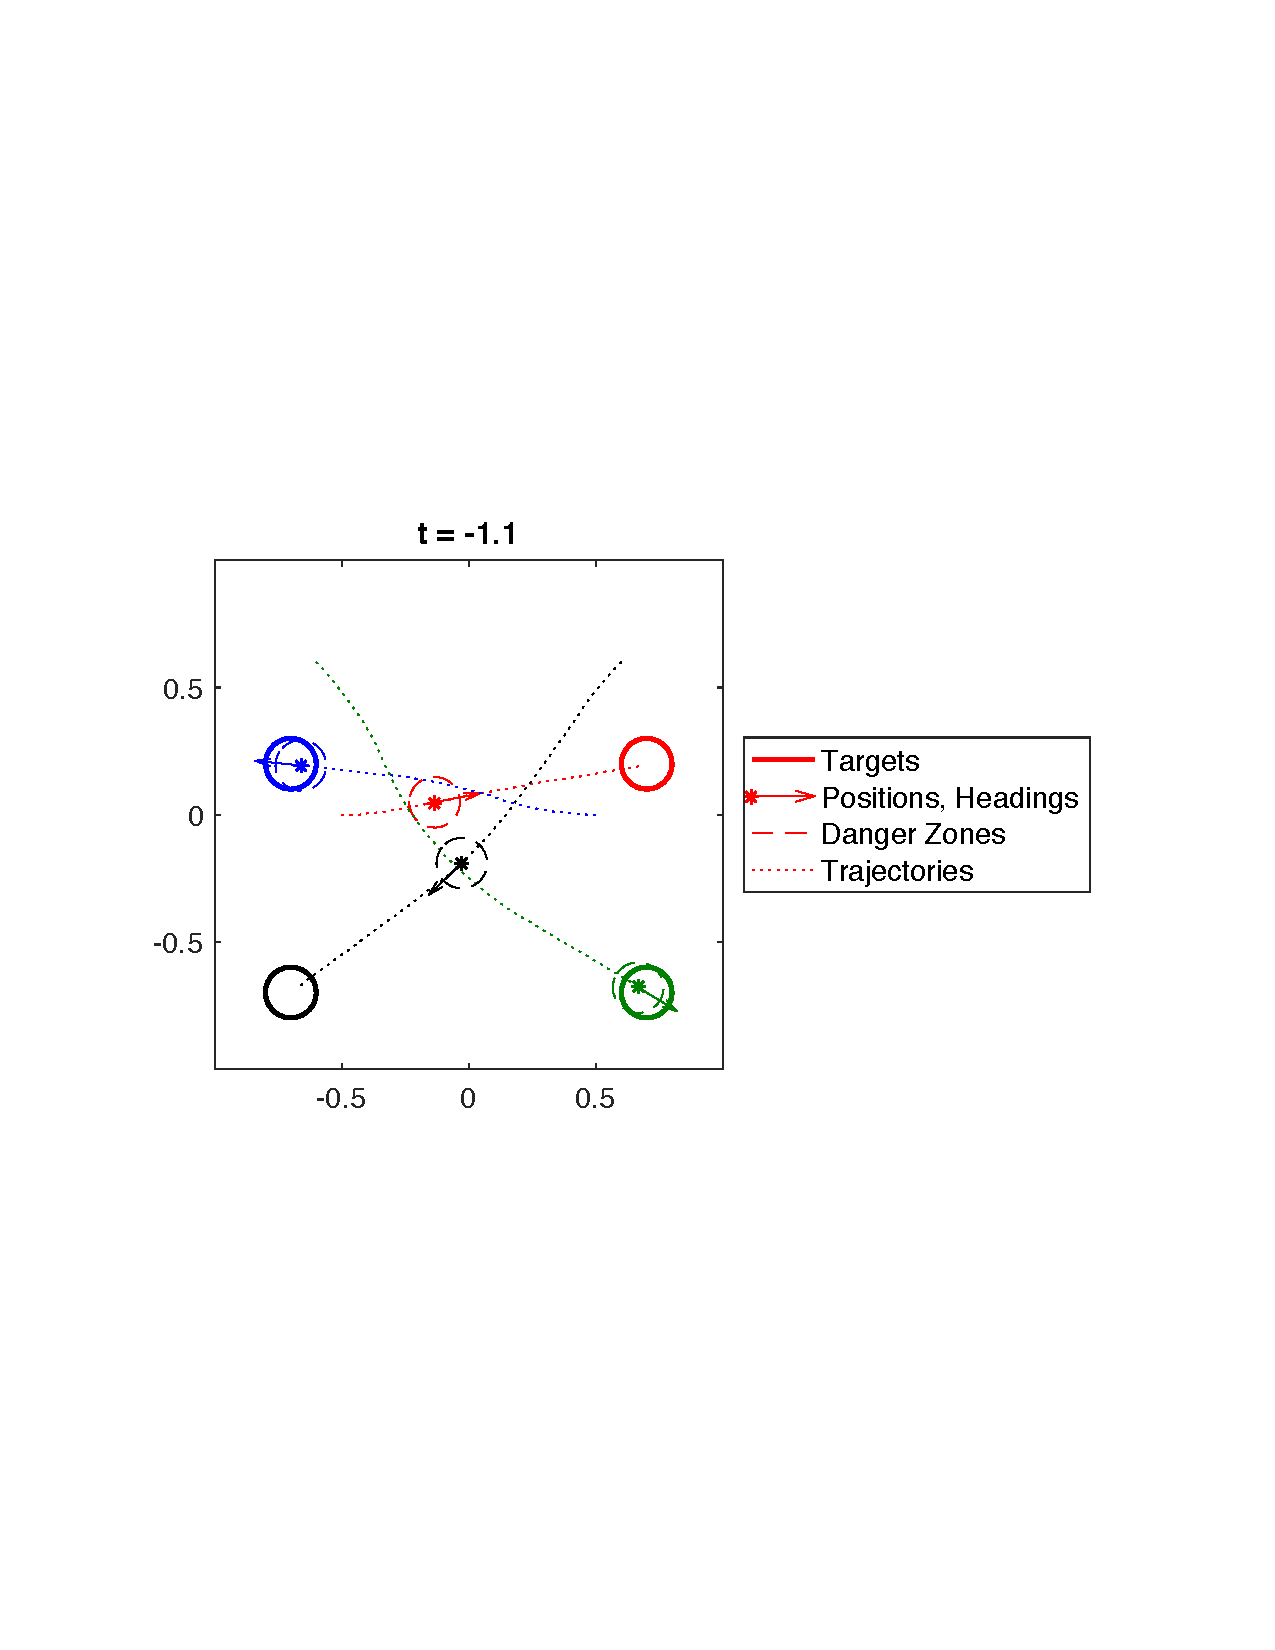
\includegraphics[width=0.8\columnwidth]{fig/rtt_traj}
  \caption{Simulated trajectories for the robust trajectory tracking method.}
  \label{fig:rtt_traj}
\end{figure}

\begin{figure}
  \centering
  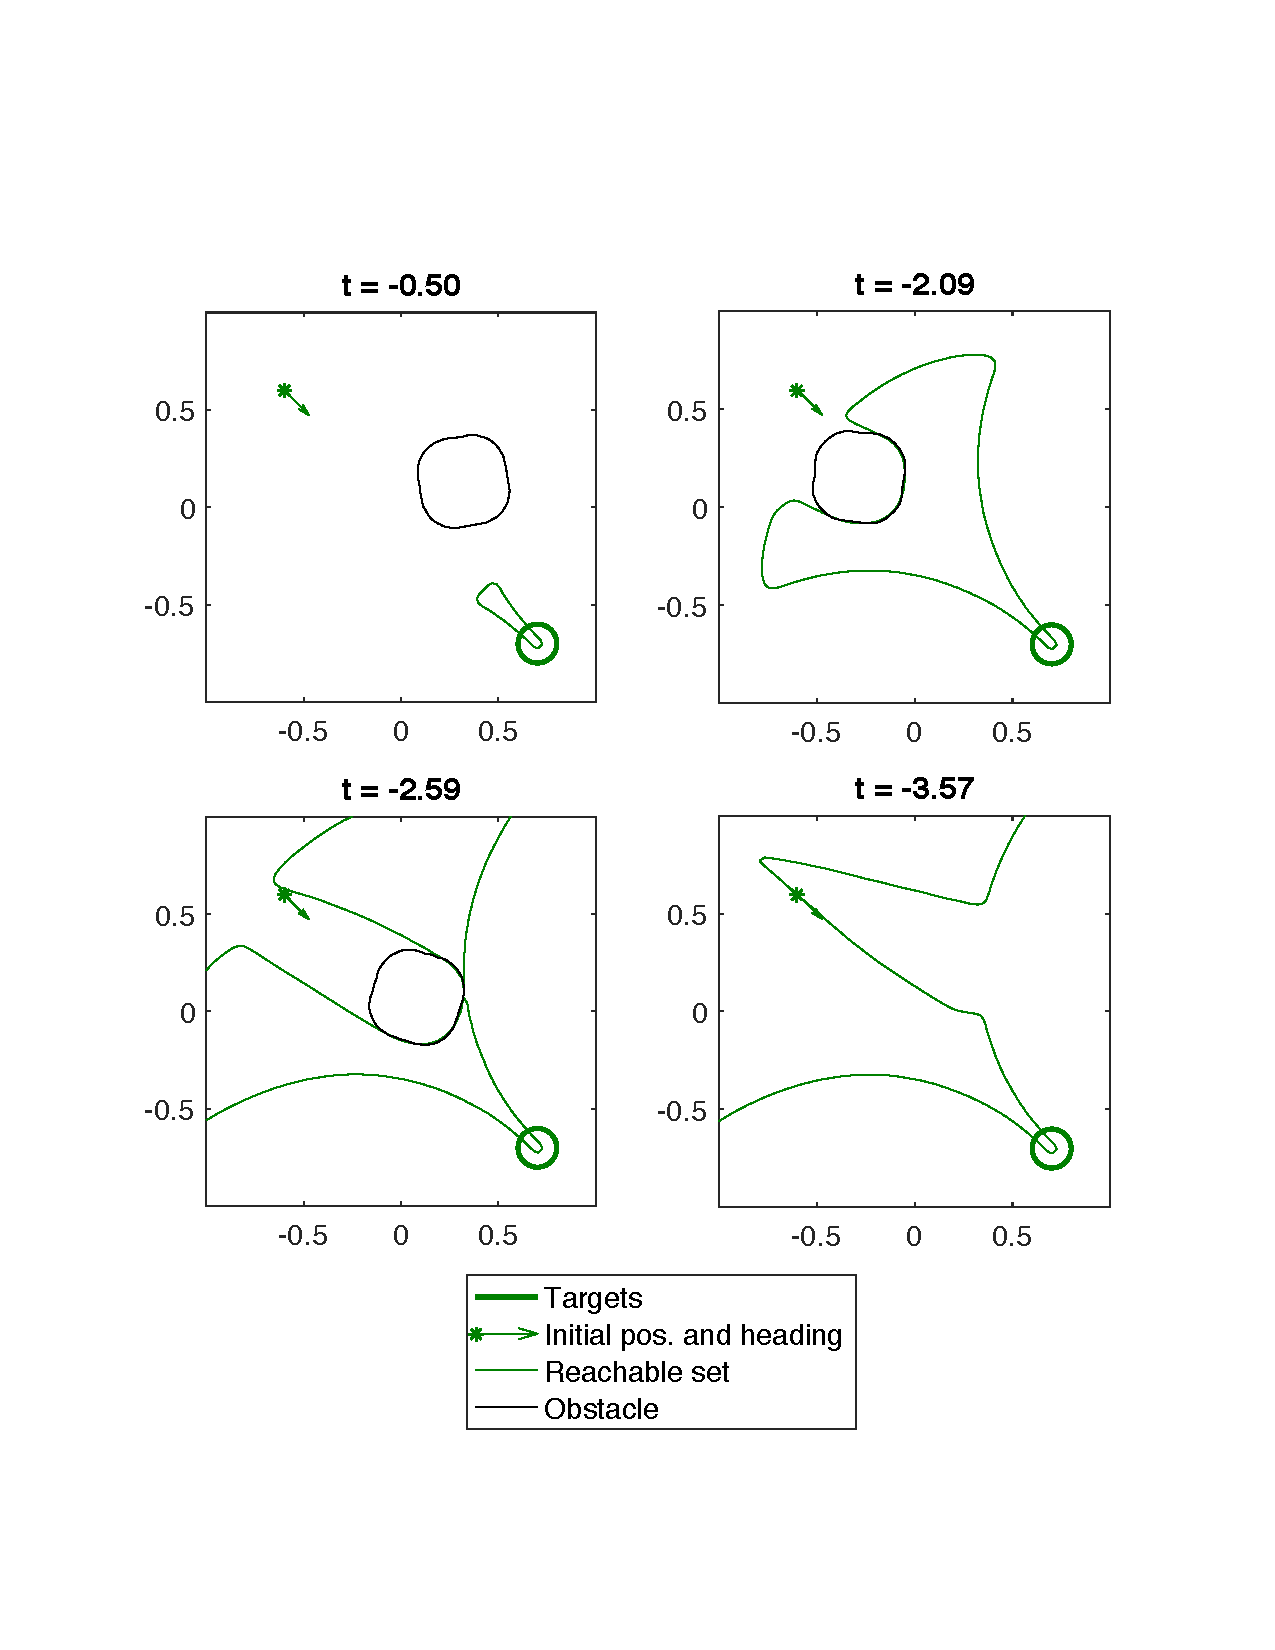
\includegraphics[width=0.9\columnwidth]{fig/rtt_rs3}
  \caption{Evolution of the BRS for $\veh_3$ in the robust trajectory tracking method. As the BRS grows in time, the induced obstacles carve out a channel. Note that a smaller target set is used to compute the BRS to ensure that the vehicle reaches the target set by $t=0$ for any allowed tracking error.}
  \label{fig:rtt_rs3}
\end{figure}

In this case, the $\ldt_i$ values for the four vehicles are $-1.61, -3.16, -3.57$ and $-2.47$ respectively. In this method, vehicles use reduced control authority for trajectory planning towards a reduced-size effective target set. As a result, higher-priority vehicles tend to have earlier $\ldt_i$'s compared to the other two methods, as evident from $\ldt_1$. Because of this ``sacrifice" made by the higher-priority vehicles during the trajectory planning phase, the $\ldt$'s of lower-priority vehicles may be later compared to those in the other methods, as evident from $\ldt_4$. Overall, it is unclear how $\ldt_i$ will change for a vehicle compared to the other methods, as the conservative trajectory planning leads to earlier $\ldt_i$'s for higher-priority vehicles and later $\ldt_i$'s for lower-priority vehicles.